\documentclass[11pt,fleqn]{article}

\setlength {\topmargin} {-.15in}
\setlength {\textheight} {8.6in}

\usepackage{amsmath}
\usepackage{amssymb}
\usepackage{amsthm}
\usepackage{url}
\usepackage{color}
\usepackage{tikz}
\usetikzlibrary{automata,positioning,arrows}

\setlength {\topmargin} {-.15in}
\setlength {\textheight} {8.6in}

\renewcommand{\labelenumi}{\theenumi.}
\renewcommand{\labelenumii}{\theenumii.}
\renewcommand{\labelenumiii}{\theenumiii.}
\newcommand{\be}{\begin{enumerate}}
	\newcommand{\ee}{\end{enumerate}}
\newcommand{\bi}{\begin{itemize}}
	\newcommand{\ei}{\end{itemize}}
\newcommand{\bc}{\begin{center}}
	\newcommand{\ec}{\end{center}}
\newcommand{\bsp}{\begin{sloppypar}}
	\newcommand{\esp}{\end{sloppypar}}
\newcommand{\mname}[1]{\mbox{\sf #1}}
\newcommand{\sB}{\mbox{$\cal B$}}
\newcommand{\sC}{\mbox{$\cal C$}}
\newcommand{\sF}{\mbox{$\cal F$}}
\newcommand{\sM}{\mbox{$\cal M$}}
\newcommand{\sP}{\mbox{$\cal P$}}
\newcommand{\sV}{\mbox{$\cal V$}}
\newcommand{\set}[1]{{\{ #1 \}}}
\newcommand{\Neg}{\neg}
\ifdefined \And
\renewcommand{\And}{\wedge}
\else
\newcommand{\And}{\wedge}
\fi
\newcommand{\Or}{\vee}
\newcommand{\Implies}{\Rightarrow}
\newcommand{\Iff}{\LeftRightarrow}
\newcommand{\Forall}{\forall}
\newcommand{\ForallApp}{\forall\,}
\newcommand{\Forsome}{\exists}
\newcommand{\ForsomeApp}{\exists\,}
\newcommand{\mdot}{\mathrel.}
\newcommand{\eps}{\epsilon}
\newcommand{\pnote}[1]{\langle \mbox{#1} \rangle}


\begin{document}

\begin{center}

{\large \textbf{COMPSCI/SFWRENG 2FA3}}\\[2mm]
{\large \textbf{Discrete Mathematics with Applications II}}\\[2mm]
{\large \textbf{Winter 2021}}\\[8mm]
{\huge \textbf{Assignment 10}}\\[6mm]
{\large \textbf{Dr.~William M. Farmer and Dr.~Mehrnoosh Askarpour}}\\[2mm]
{\large \textbf{McMaster University}}\\[6mm]
{\large Revised: March 29, 2021}

\end{center}

\medskip

Assignment 10 consists of two problems.  You must write your solutions
to the problems using LaTeX.

Please submit Assignment~10 as two files,
\texttt{Assignment\_10\_\emph{YourMacID}.tex} and
\texttt{Assignment\_10\_\emph{YourMacID}.pdf}, to the Assignment~10
folder on Avenue under Assessments/Assignments.
\texttt{\emph{YourMacID}} must be your personal MacID (written without
capitalization).  The \texttt{Assignment\_10\_\emph{YourMacID}.tex}
file is a copy of the LaTeX source file for this assignment
(\texttt{Assignment\_10.tex} found on Avenue under
Contents/Assignments) with your solution entered after each problem.
The \texttt{Assignment\_10\_\emph{YourMacID}.pdf} is the PDF output
produced by executing

\begin{itemize}

  \item[] \texttt{pdflatex Assignment\_10\_\emph{YourMacID}}

\end{itemize}

This assignment is due \textbf{Sunday, April 11, 2021 before
  midnight.}  You are allow to submit the assignment multiple times,
but only the last submission will be marked.  \textbf{Late submissions
  and files that are not named exactly as specified above will not be
  accepted!}  It is suggested that you submit your preliminary
\texttt{Assignment\_10\_\emph{YourMacID}.tex} and
\texttt{Assignment\_10\_\emph{YourMacID}.pdf} files well before the
deadline so that your mark is not zero if, e.g., your computer fails
at 11:50 PM on April 11.

\textbf{Although you are allowed to receive help from the
  instructional staff and other students, your submission must be your
  own work.  Copying will be treated as academic dishonesty! If any of
  the ideas used in your submission were obtained from other students
  or sources outside of the lectures and tutorials, you must
  acknowledge where or from whom these ideas were obtained.}

\newpage

\subsection*{Problems}

\be

  \item \textbf{[4 points]} Recall the diagonalization argument used
    in the Week 12 Exercises to show that the set of real numbers in
    the interval $[0,1]$ is uncountable.  If we tried to use this same
    argument to show that the set of rational numbers in the interval
    $[0,1]$ is uncountable, where and why would the argument fail?

  \bigskip

  \textcolor{blue}{\textbf{Mohammad Omar Zahir, zahirm1, April 11, 2021}}

  To show that the argument fails for showing that the set of rational numbers in the [0, 1] interval is uncountable, we must revisit why the set of real numbers in the interval was uncountable. Diagonalization was applied to prove that there exist an infinte number of values in the interval, through the use of a table which mapped functions to everu real number to a function. We used the following structure in our diagnolization.\\
  
  $x_1x_2x_3...x_n \: \mname{where}\:  x_i  \in  \{1 \: \mname{when} \: y_i = 0, \: \mname{and} \: 0 \: \mname{when} \: y_i = 1\}$\\
  
  Here $x_i$ represents the complements of the diagonals in the table, where we are assuming that the $x_i$ is not in the table, meaning it has not yet been counted. If it happens that we put the element in, that implies that you would be creating another element that has not yet been counted. If this pattern is maintained, we can see that there will be an infinite number of elements, and thus not countable.\\
  
  This is the part of the proof that fails for rational numbers as there is no way to know that the numbers that are being added are indeed rational, as they could also be irrational, meaning it can not be represented in the form of a fraction. An irrational number such as this would thus not be represented in the diagonalization and not be mapped to a function as this number would not belong from the set that we are trying to prove uncountable. This, hence, fails the proof.
    
  \item Let $\Sigma$ be a finite alphabet and $A,B \subseteq \Sigma^*$
    be r.e.~sets.

  \be

    \item\textbf{[8 points]} Prove that $A \cup B$ is r.e.

    \bigskip

    \textcolor{blue}{\textbf{Mohammad Omar Zahir, zahirm1, April 11, 2021}}

    As per the question we will take the sets A and B, and let them be accepted by the following two turing machines, M1 and M2. We will then let A $\cup$ B represent the turing machine M that contains the two turing machine M1 and M2, as shown in the diagram below. We will then let $x$ represent the input to this turing machine such that $x = a_1 \cup a_2$ where $a_1 \in A$ and $a_2 \in b$. We will then need to run both the M1 and M2 turing machines simultaneously to check if either of them accept the input $x$. To process this we will need to simulate the turing machine M as a two-tape turing machine where M1 is processed on the first tape and M2 is processed on the second.\\\\
    We know that because $M$ represents the union of the two r.e sets, if either of the two turing machines enters their respective accept states for the word $x$, the turing machine $M$ will also accept it. This is because union will take all the accepted inputs from both machines and allow it to be the accepted input for $M$. Unlike acceptance, however, for rejection both turing machines must reject the word for the word to be rejected by $M$, otherwise it would be present in the union set if it is accepted by one machine, and will then be accepted by $M$ as a whole. Similar to the acceptance, if one turing machine loops on an input, then the turing machine $M$ will also loop on the input. However, if one accepts and one loops, then the turing machine $M$ will accept the input rather than loop. Therefore since we have defined and shown that the turing machine $M$ can accept $A\cup B$, we know that $A\cup B$ is an r.e.
    
    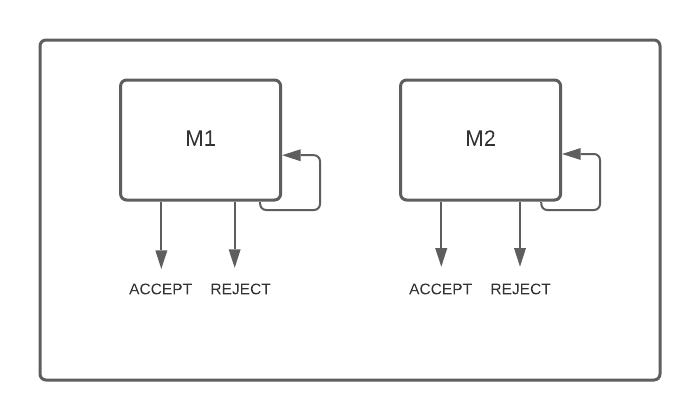
\includegraphics[width=0.8\textwidth]{FA3_Turing_Machine .png} \\

    \medskip

    \item\textbf{[8 points]} Prove that $A \cap B$ is r.e.

    \bigskip

    \textcolor{blue}{\textbf{Mohammad Omar Zahir, zahirm1, April 11, 2021}}
    
    Similar to part a, we will take the sets A and B, and let them be accepted by the following two turing machines, $M_1$ and $M_2$. We will then let A $\cap$ B represent the turing machine M that contains the two turing machine $M_1$ and $M_2$, as shown in the diagram below. We will then let $x$ represent the input to this turing machine such that $x = a_1 \cup a_2$ where $a_1 \in A$ and $a_2 \in b$. We will then need to run both the $M_1$ and $M_2$ turing machines simultaneously to check if either of them accept the input $x$. To process this we will need to simulate the turing machine $M$ as a two-tape turing machine where $M_1$ is processed on the first tape and $M_2$ is processed on the second.\\\\
    
    We know that because $M$ represents the intersection of the two r.e sets, if either of the two turing machines enter their respective accept states for the word $x$, that does not necessarily imply that the turing machine $M$ will also accept it. This is because intersection only returns those inputs that are accepted by both turing machines, and if one does not accept a word, then it will not show up for the entire turing machine $M$. This does not affect the rejection of these states, however, because if one turing machine accepts the word, and one rejects it, it will not be accepted by the whole turing machine since the word is not in both sets. That is to say that if one turing machine rejects a word then $M$ will also reject it. Similar to the acceptance for intersection, if the turing machine $M$ loops on an input then that would mean that both turing machines $M_1$ and $M_2$ would also need to loop on it, due to intersection. Therefore since we have defined and shown that the turing machine $M$ can accept $A\cup B$, we know that $A \cap B$ is an r.e.
    
    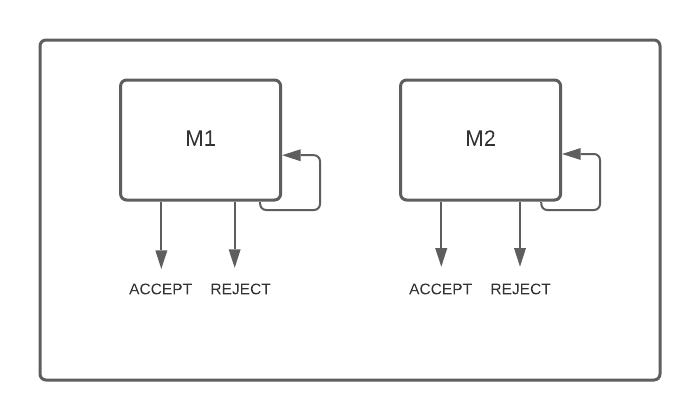
\includegraphics[width=0.8 \textwidth]{FA3_Turing_Machine .png} \\


  \ee

  \bigskip

\ee

\end{document}
